% 2019 上海春季卷第 10 题；取 a=2 作示意，曲线、交点依题设计算。
% 图形比例为排版示意，不对应源图物理尺寸。
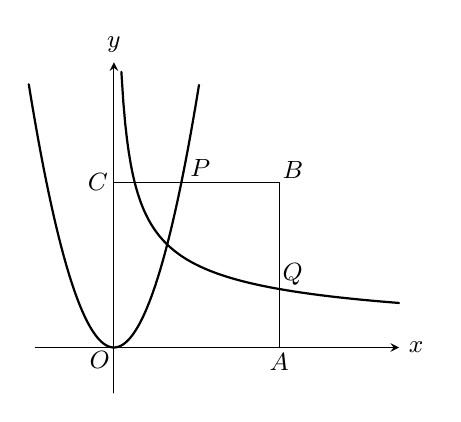
\begin{tikzpicture}[x=1.05cm,y=1.05cm,line cap=round,line join=round,>=stealth,font=\small]
  \coordinate (O) at (0,0);
  \coordinate (A) at (2,0);
  \coordinate (B) at (2,2);
  \coordinate (C) at (0,2);
  \coordinate (P) at ({sqrt(2/3)},2);
  \coordinate (Q) at (2,{1/sqrt(2)});

  \draw[->] (-0.95,0) -- (3.45,0) node[right] {$x$};
  \draw[->] (0,-0.55) -- (0,3.45) node[above] {$y$};
  \draw (C) -- (B) -- (A);
  \draw[thick,domain=-1.03:1.03,samples=90] plot (\x,{3*\x*\x});
  \draw[thick,domain=0.09:3.45,samples=150] plot (\x,{1/sqrt(\x)});

  \node[below left,inner sep=1.3pt] at (O) {$O$};
  \node[below,inner sep=2pt] at (A) {$A$};
  \node[above right,inner sep=1pt] at (B) {$B$};
  \node[left,inner sep=2pt] at (C) {$C$};
  \node[above right,xshift=2pt,yshift=1pt,inner sep=1pt] at (P) {$P$};
  \node[above right,inner sep=1pt] at (Q) {$Q$};
\end{tikzpicture}
